\documentclass[11pt]{article}
\usepackage{amsmath}
\usepackage{graphicx}
\usepackage{hyperref}
\usepackage[utf8]{inputenc}
\usepackage[spanish]{babel}
\usepackage[margin=2.5cm]{geometry}
\usepackage{amsfonts}
\usepackage{listings}
\usepackage[T1]{fontenc}
\usepackage{float}
\usepackage{subfig}
\usepackage{textcomp}

\title{Trabajo 4 - Análisis de latidos.}
\author{Néstor Rodríguez Vico. DNI: 75573052C - \href{mailto:nrv23@correo.ugr.es}{nrv23@correo.ugr.es} \\ Míriam Mengíbar Rodríguez. DNI: 20227044Q - \href{mailto:mirismr@correo.ugr.es}{mirismr@correo.ugr.es}}
\date{\today}


\lstdefinestyle{bash_style}{
	language=MatLab,
	frame=single,
	xleftmargin=.25in,
	upquote = true,
	basicstyle=\scriptsize,
	breakatwhitespace=false,         
	breaklines=true,                 
	captionpos=b,                    
	keepspaces=true,                 
	numbers=left,                    
	numbersep=5pt,                  
	showspaces=false,                
	showstringspaces=false,
	showtabs=false,                  
	tabsize=2,
	upquote=true
}

\lstset{style=bash_style}

\begin{document}

\maketitle

\setlength{\belowdisplayskip}{5pt} 
\setlength{\belowdisplayshortskip}{5pt}
\setlength{\abovedisplayskip}{5pt} 
\setlength{\abovedisplayshortskip}{5pt}

\section{Solución.}

Para resolver el ejercicio nos hemos basado en el código proporcionado en la asignatura. Los pasos seguidos han sido:

\begin{enumerate}
	\item Calculamos la media para cada banda de color para cada frame. De esta manera vamos a tener una matriz con 3 medias para cada frame, una para cada banda. Guardamos dichas medias en una única matriz.
	\item A continuación, normalizamos las medias. Para ello, le restamos la media y lo dividimos por su desviación.
	\item A continuación, multplicamos nuestra matriz de medias por su transpuesta, para tener una matriz \textit{3x3}. Dicha matriz la denotaremos como \textit{X}.
	\item Ahora calculamos los autovalores y autovectores de la matriz \textit{X} y nos quedamos con el autovector cuyo autovalor correspondientes es máximo.
	\item Finalmente, aplicamos la fórmula \textit{y=mejor autovector * (X - media(X))}. La \textit{y} es la salida de nuestra función.
\end{enumerate}

A continuación se muestra el código desarrollado:

\begin{lstlisting}
function signal = acquire_RGB(video)
	numFrames = video.NumberOfFrames;
	means_R = zeros(1, numFrames);
	means_G = zeros(1, numFrames);
	means_B = zeros(1, numFrames);
	
	for i=1:numFrames
		frame = read(video, i);
		% Obtenemos la media de cada banda
		means_R(i)=sum(sum(frame(:,:,1)))/(size(frame,1)*size(frame,2));
		means_G(i)=sum(sum(frame(:,:,2)))/(size(frame,1)*size(frame,2));
		means_B(i)=sum(sum(frame(:,:,3)))/(size(frame,1)*size(frame,2));
	end
	
	% Guardamos las medias en una matriz
	means = transpose([means_R; means_G; means_B]);
	norm_means_R=transpose((means(:,1)-mean(means(:,1)))/std(means(:,1)));
	norm_means_G=transpose((means(:,2)-mean(means(:,2)))/std(means(:,2)));
	norm_means_B=transpose((means(:,3)-mean(means(:,3)))/std(means(:,3)));
	means_standar=transpose([norm_means_R; norm_means_G; norm_means_B]);
	
	% Y la multiplicamos por su traspuesta, asi tenemos una matriz [3 3]
	X = transpose(means_standar) * means_standar;
	% Calculamos sus autovalores y autovectores
	[V, D] = eig(X);
	% Ordenamos los autovalores de mayor a menos valor
	[~, idx] = sort(diag(D), 'descend');
	% El mejor autovector es el correspontiende al autovalor mas grande
	best = transpose(V(:,idx(1)));
	% Aplicamos la formula signal=autovector*(X-media(X))
	signal = best*(transpose(means_standar)-mean(means_standar(:)));
end
\end{lstlisting}

\section{Resultados.}

El resultado para el vídeo proporcionado es el siguiente:

\begin{figure}[H]
	\centering
	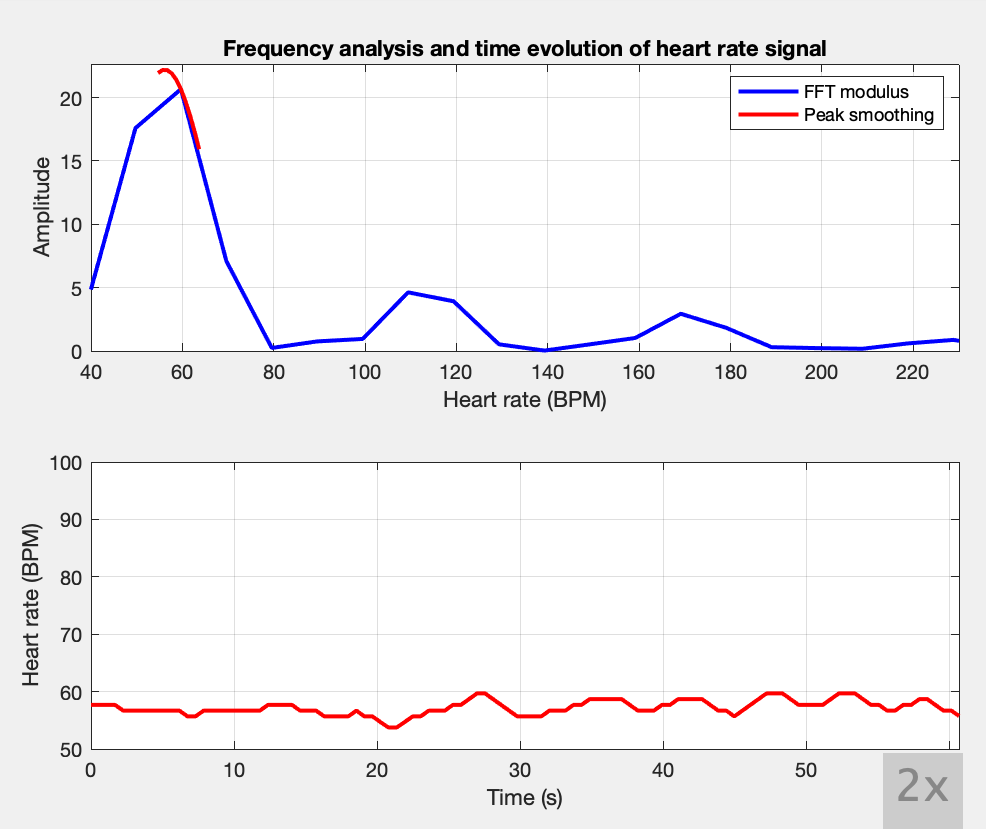
\includegraphics[width=0.7\textwidth]{images/originalRGB.png}
\end{figure}

Si comparamos ambas señales, obtenemos un \textit{psnr} de \textit{9.0067} y un \textit{mse} de \textit{8173.6}. En el caso de usar sólo la banda de color rojo obtenemos unos latidos por minuto medios de \textit{57.2418}, mientras que si usamos las tres bandas obtenemos un valor de \textit{57.2244}. \\

A continuación se muestran los resultados de un hombre de 25 años con actividad física media-baja:

\begin{table}[H]
	\centering
	\begin{tabular}{cc}
		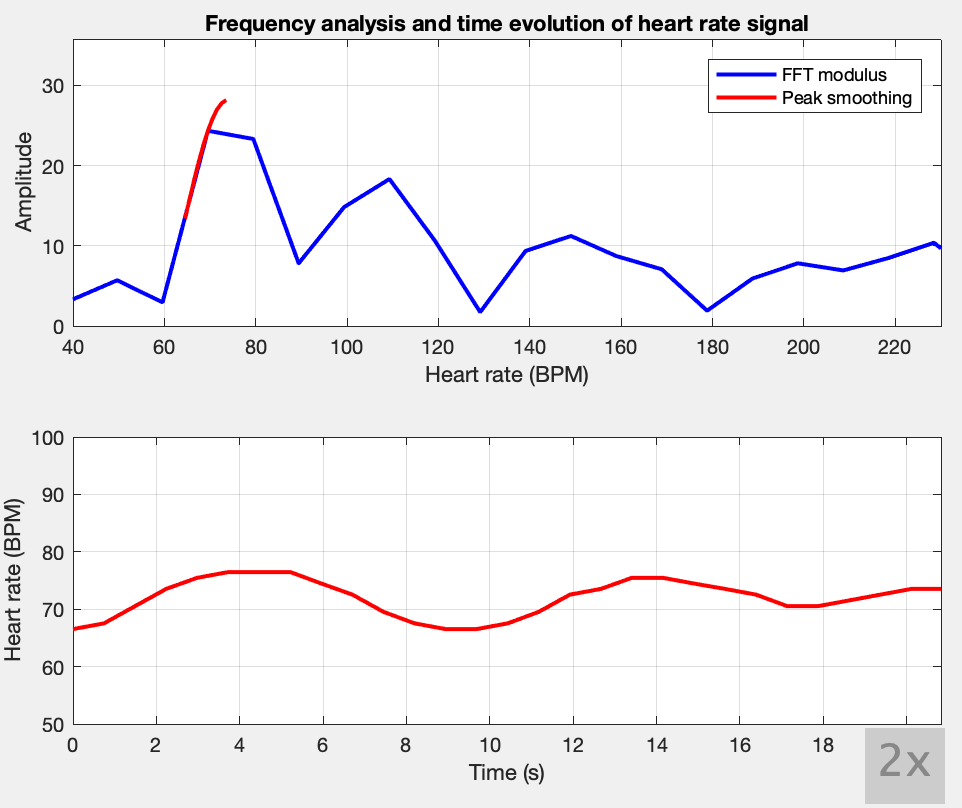
\includegraphics[width=0.5\textwidth]{images/sujeto1_R.png} & 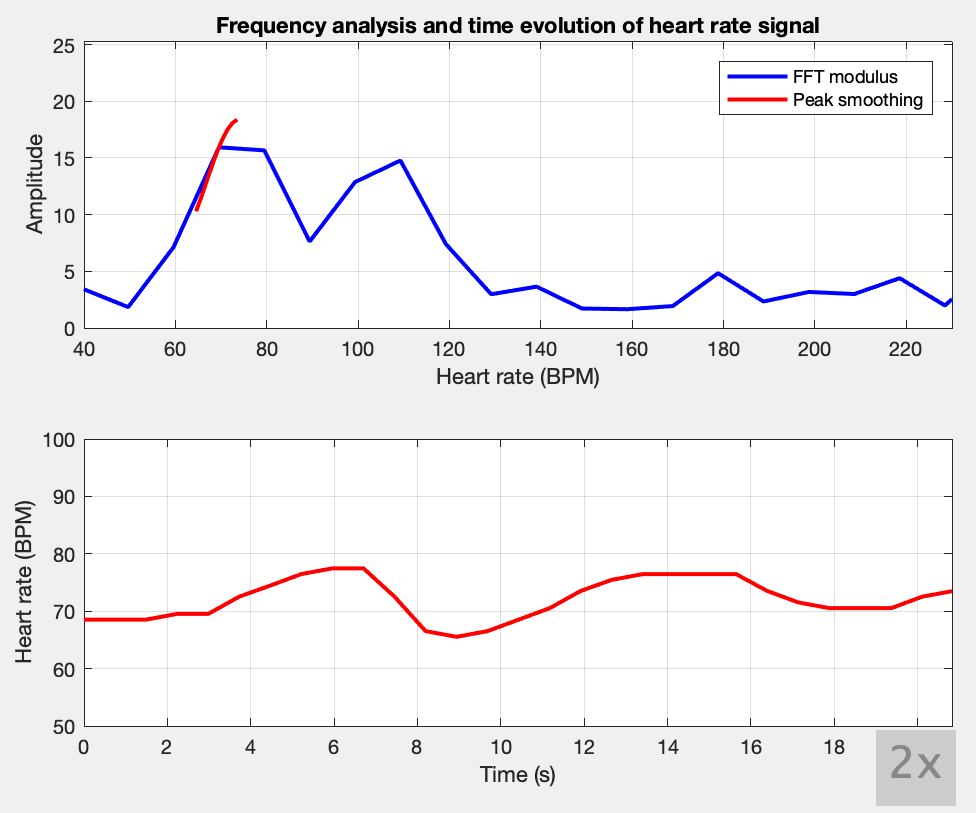
\includegraphics[width=0.5\textwidth]{images/sujeto1_RGB.png}
	\end{tabular}
\end{table}

A la izquierda tenemos el resultado de usar sólo la banda de color rojo y a la derecha el resultado de usar las tres bandas de color. En el caso de usar sólo la banda de color rojo obtenemos unos latidos por minuto medios de \textit{70.0159}, mientras que si usamos las tres bandas obtenemos un valor de \textit{71.2188}. Si comparamos ambas señales, obtenemos un \textit{psnr} de \textit{13.0788} y un \textit{mse} de \textit{3200.4}. Aquí podemos ver que hay más simulitud entre ambas señales con respecto al experimento anterior, ya que tenemos un \textit{psnr} más alto y un \textit{mse} más bajo. En este caso, quizás no nos interesa el gasto computacional de usar las tres bandas con respecto a usar sólo una de ellas. \\

A continuación se muestran los resultados de una mujer de 40 años con actividad física media:

\begin{table}[H]
	\centering
	\begin{tabular}{cc}
		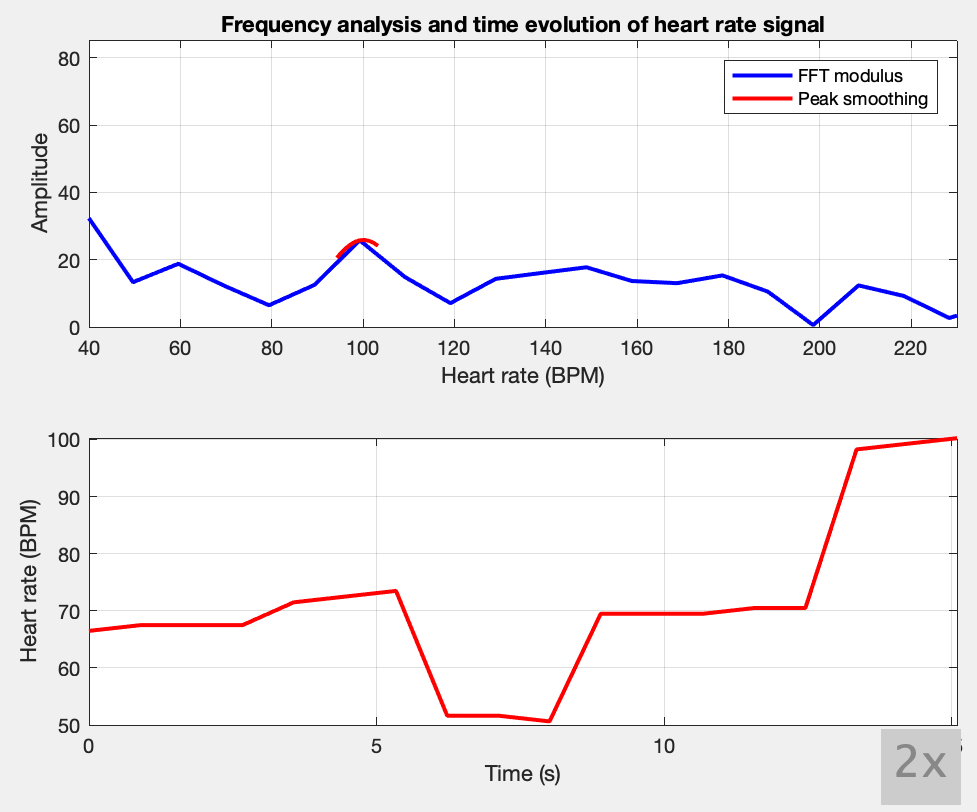
\includegraphics[width=0.5\textwidth]{images/sujeto2_R.png} & 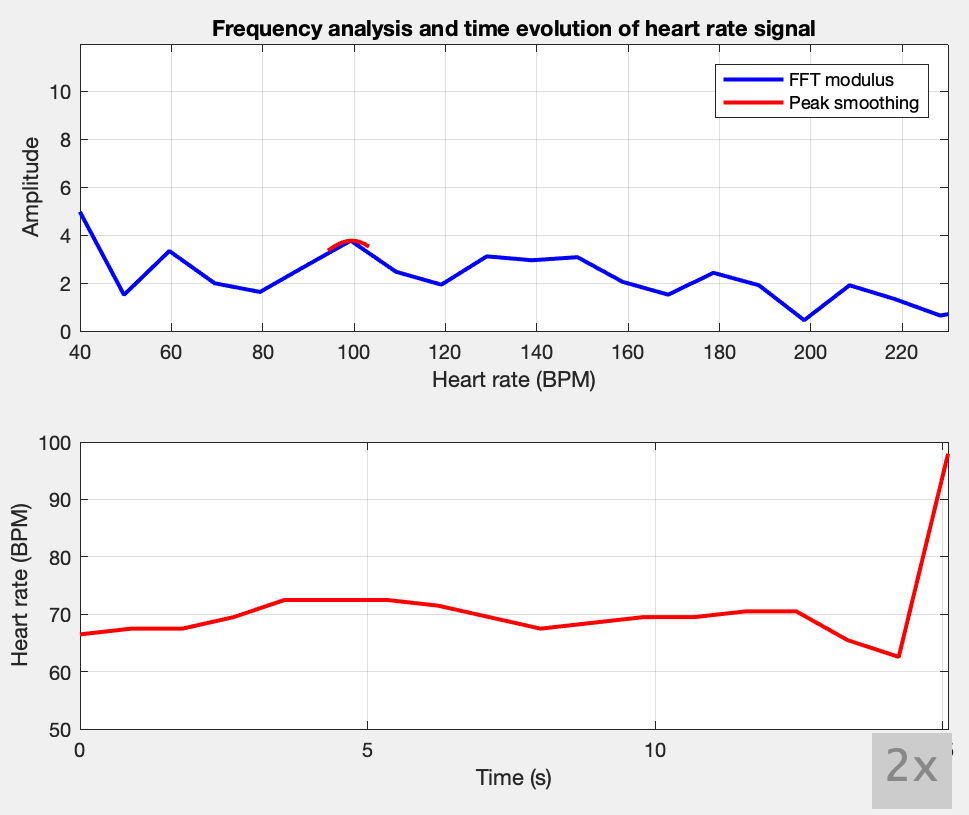
\includegraphics[width=0.5\textwidth]{images/sujeto2_RGB.png}
	\end{tabular}
\end{table}

Justo al final del experimento le hemos dado un susto para ver como se comportaban los latidos de su corazón, y podemos verlo reflejado en las gráficas. A la izquierda tenemos el resultado de usar sólo la banda de color rojo y a la derecha el resultado de usar las tres bandas de color. En el caso de usar sólo la banda de color rojo obtenemos unos latidos por minuto medios de \textit{71.5254}, mientras que si usamos las tres bandas obtenemos un valor de \textit{70.6962}. Si comparamos ambas señales, obtenemos un \textit{psnr} de \textit{5.0578} y un \textit{mse} de \textit{20291}. En este caso, si hay bastante diferencia entre ambas señales, ya que el \textit{psnr} es muy bajo y el \textit{mse} muy alto. En este caso, si nos puede interesar usar las tres bandas. \\

A continuación se muestran los resultados de una mujer de 23 años con actividad física media:

\begin{table}[H]
	\centering
	\begin{tabular}{cc}
		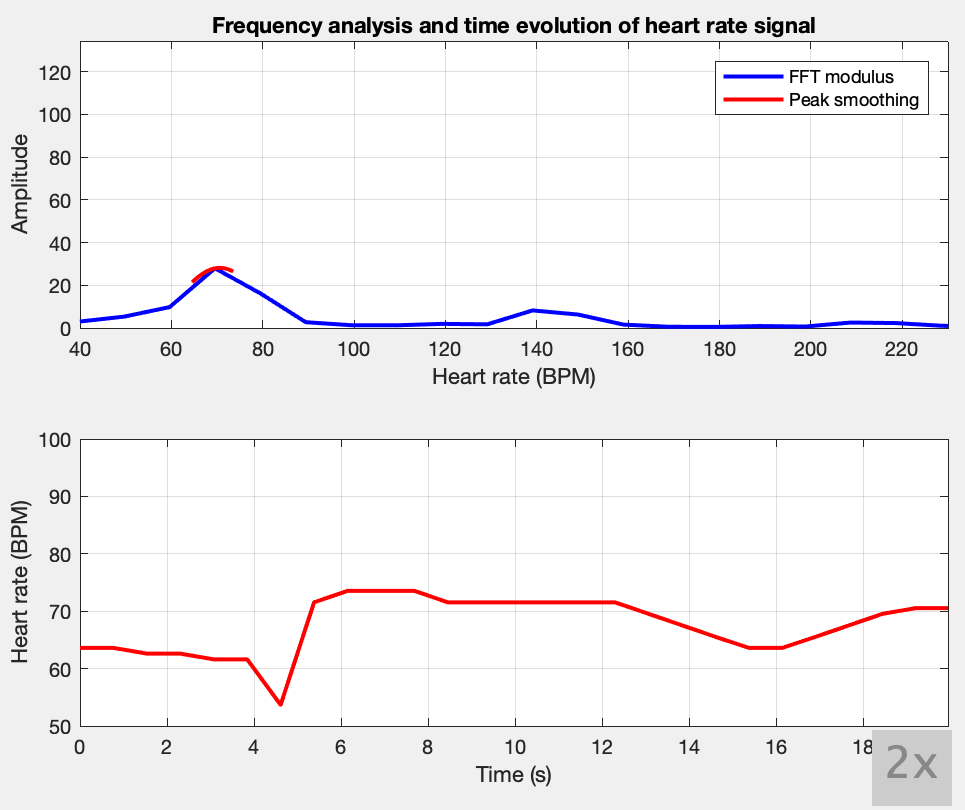
\includegraphics[width=0.5\textwidth]{images/sujeto3_R.png} & 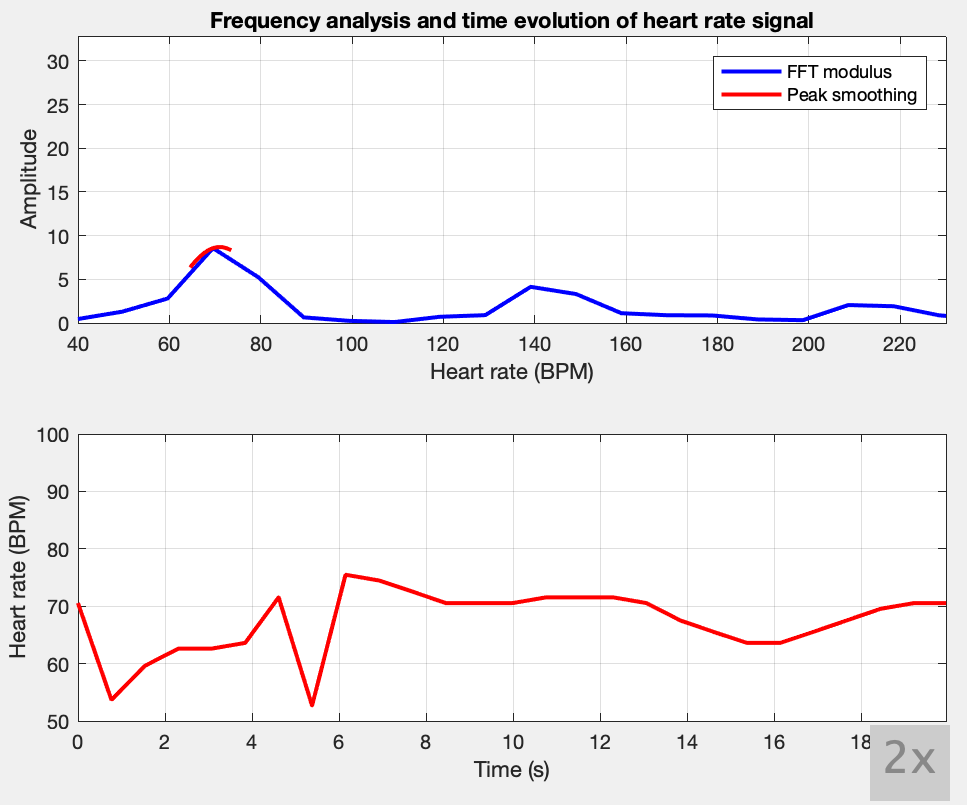
\includegraphics[width=0.5\textwidth]{images/sujeto3_RGB.png}
	\end{tabular}
\end{table}

A la izquierda tenemos el resultado de usar sólo la banda de color rojo y a la derecha el resultado de usar las tres bandas de color. En el caso de usar sólo la banda de color rojo obtenemos unos latidos por minuto medios de \textit{67.5679}, mientras que si usamos las tres bandas obtenemos un valor de \textit{67.4149}. Si comparamos ambas señales, obtenemos un \textit{psnr} de \textit{10.9930} y un \textit{mse} de \textit{5173.4}. Aquí podemos ver que hay más simulitud entre ambas señales, ya que tenemos un \textit{psnr} más alto y un \textit{mse} más bajo. En este caso, quizás no nos interesa el gasto computacional de usar las tres bandas con respecto a usar sólo una de ellas. \\

A continuación se muestran los resultados la misma persona que en el experimento anterior pero justo después de salir a hacer deporte:

\begin{table}[H]
	\centering
	\begin{tabular}{cc}
		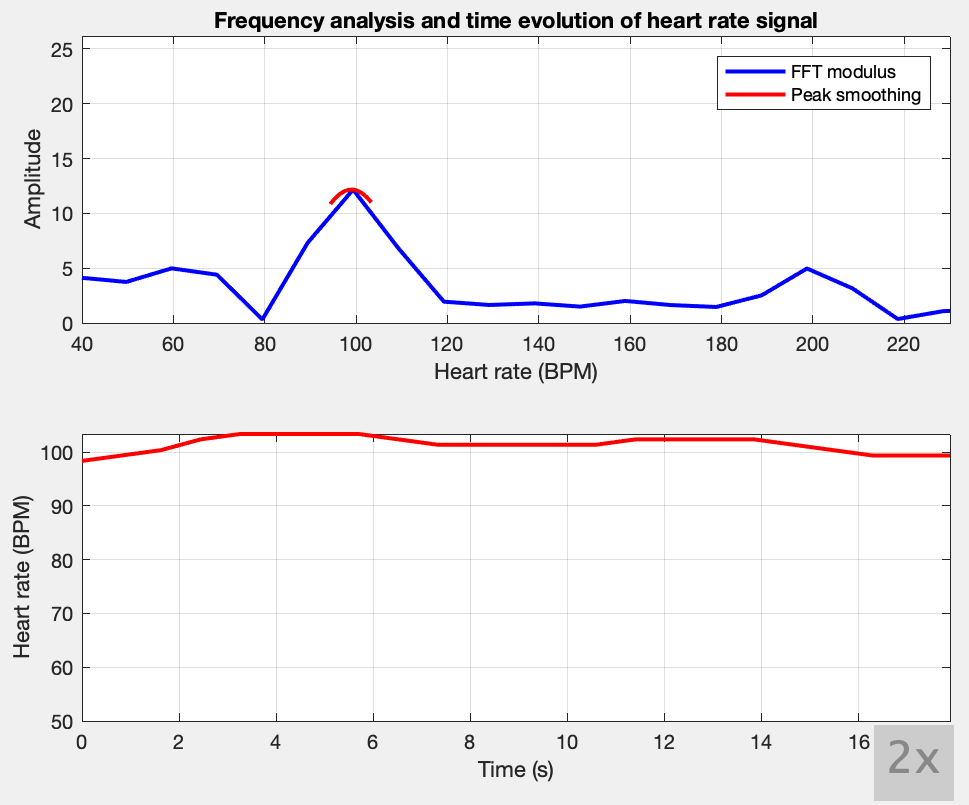
\includegraphics[width=0.5\textwidth]{images/sujeto4_R.png} & 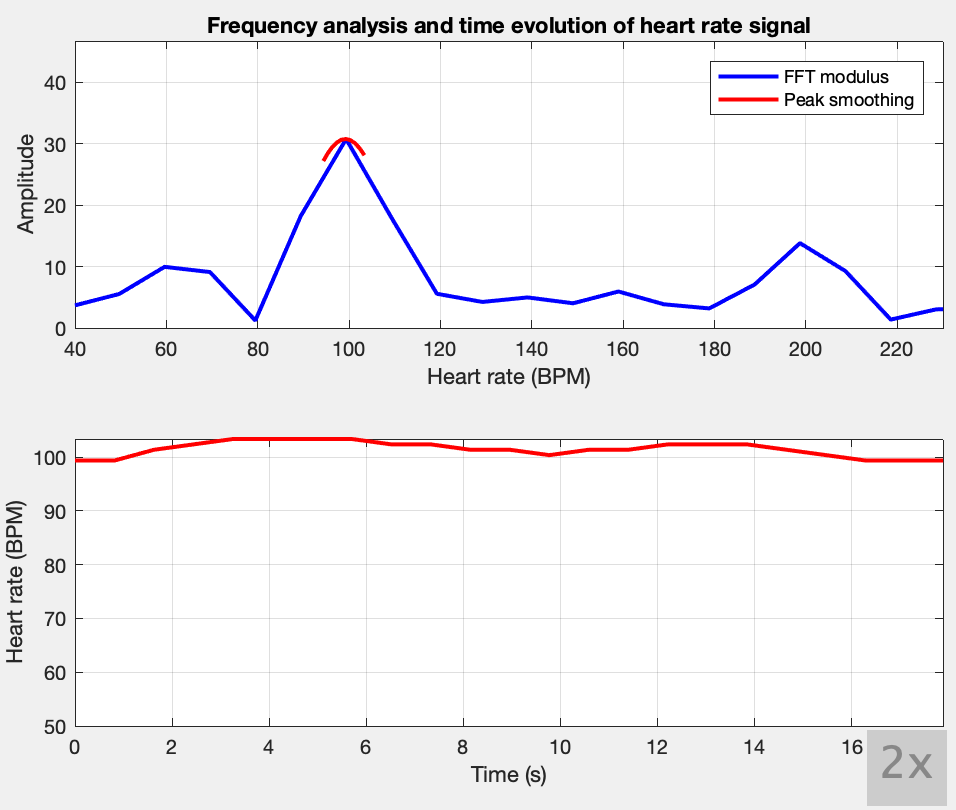
\includegraphics[width=0.5\textwidth]{images/sujeto4_RGB.png}
	\end{tabular}
\end{table}

A la izquierda tenemos el resultado de usar sólo la banda de color rojo y a la derecha el resultado de usar las tres bandas de color. En el caso de usar sólo la banda de color rojo obtenemos unos latidos por minuto medios de \textit{101.3916}, mientras que si usamos las tres bandas obtenemos un valor de \textit{101.4351}. Si comparamos ambas señales, obtenemos un \textit{psnr} de \textit{13.4949} y un \textit{mse} de \textit{2908}. Aquí podemos ver que hay más simulitud entre ambas señales, ya que tenemos un \textit{psnr} más alto y un \textit{mse} más bajo. En este caso, quizás no nos interesa el gasto computacional de usar las tres bandas con respecto a usar sólo una de ellas. \\

A continuación se muestran los resultados de una mujer de 35 años con actividad física bajo:

\begin{table}[H]
	\centering
	\begin{tabular}{cc}
		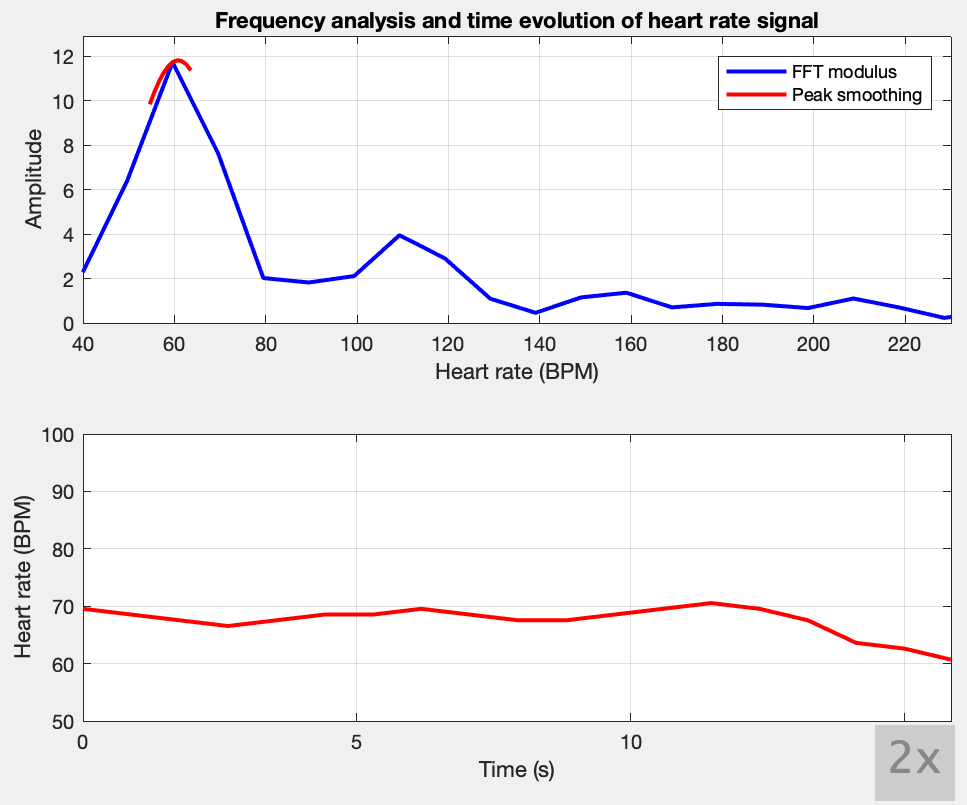
\includegraphics[width=0.5\textwidth]{images/sujeto5_R.png} & 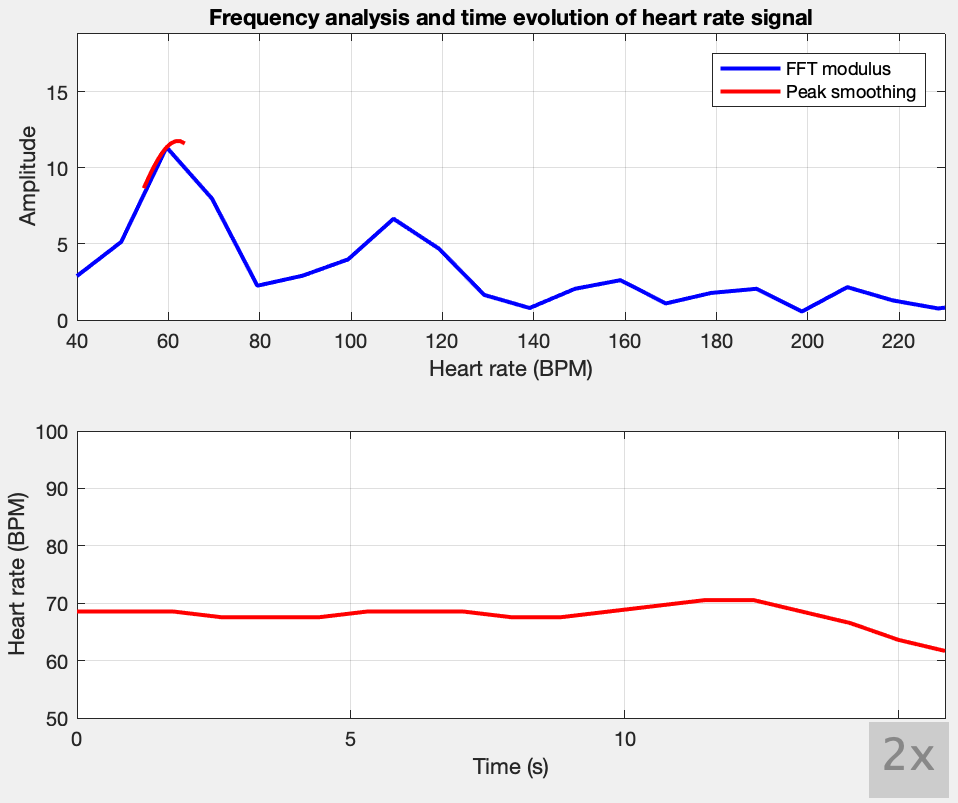
\includegraphics[width=0.5\textwidth]{images/sujeto5_RGB.png}
	\end{tabular}
\end{table}

A la izquierda tenemos el resultado de usar sólo la banda de color rojo y a la derecha el resultado de usar las tres bandas de color. En el caso de usar sólo la banda de color rojo obtenemos unos latidos por minuto medios de \textit{67.8137}, mientras que si usamos las tres bandas obtenemos un valor de \textit{67.5014}. Si comparamos ambas señales, obtenemos un \textit{psnr} de \textit{13.0530} y un \textit{mse} de \textit{3219.4}. Aquí podemos ver que hay más simulitud entre ambas señales, ya que tenemos un \textit{psnr} más alto y un \textit{mse} más bajo. En este caso, quizás no nos interesa el gasto computacional de usar las tres bandas con respecto a usar sólo una de ellas.

\section{Resultados finales.}

En esta sección vamos a comparar los latidos por minuto medios de cada sujeto. Los resultados obtenidos son:

\begin{table}[H]
	\centering
	\begin{tabular}{rcc}
		\textbf{} & \textbf{R} & \textbf{RGB} \\ \hline
		\textbf{Original} & 57.2418 & 57.2244 \\
		\textbf{Sujeto 1} & 70.0159 & 71.2188 \\
		\textbf{Sujeto 2} & 71.5254 & 70.6962 \\
		\textbf{Sujeto 3} & 67.567 & 67.4149 \\
		\textbf{Sujeto 4} & 101.391 & 101.4351 \\
		\textbf{Sujeto 5} & 67.813 & 67.5014
	\end{tabular}
\end{table}

Finalmente, si consideramos los latidos por minutos de la banda roja como una matriz de resultados y consideramos los latidos por minutos de las tres bandas como otra matriz de resultados y calculamos el error entre ambas obtenemos un \textit{psnr} de \textit{52.3757} y un \textit{mse} de \textit{0.3763}. Obtenemos un \textit{psnr} bastante alto y un \textit{mse} bastante bajo, así que podríamos decir que no se produce una mejora al usar las tres bandas de color mientras que si supone un coste computacional. Así que, podríamos conformarnos con los resultados de usar una única banda de color.

\end{document}